
\chapter{Introducción\label{intro}}

\section{Motivación\label{motivacion}}

Internet-of-Things (IoT) y las tecnologías Big Data han producido
avances significativos en el dominio de los sistemas de gestión de
flotas de vehículos. El paradigma IoT ha permitido mejorar el proceso
de seguimiento y monitorización de vehículos y las técnicas Big Data
son muy apropiadas para el análisis en tiempo real de la gran cantidad
de datos obtenidos en este proceso\cite{1-1-3}. De este modo, han
surgido nuevas aplicaciones de gestión de flotas que gestionan mejor
los recursos de la empresa y ofrecen un procesamiento más sofisticado
y escalable en sus diferentes escenarios.


Las aplicaciones de gestión de flotas son, por tanto, un dominio
apropiado para la aplicación de arquitecturas Big Data. El seguimiento
de los vehículos genera un gran volumen de datos que, a través de
diferentes técnicas de análisis de datos, podemos extraer información
de gran interés para las empresas dedicadas a este sector. Dado que
las aplicaciones de gestión de flotas, deben procesar esta gran
cantidad de datos y proporcionar diferentes beneficios, las
tecnologías Big Data son muy apropiadas para tratarlos. Algunos de los
beneficios que podemos obtener con este tipo de aplicaciones es
reducir el coste de gestionar la flota, ser más responsable con el
medio ambiente y poder controlar cualquier tipo de robo o mal uso de
los vehículos de la empresa propietaria de la flota \cite{1-1-1,1-1-2}.

\mdata\footnote{\url{https://movildata.com/sobre-nosotros/}.} es
una empresa con sede en Murcia dedicada a ofrecer soluciones para la
gestión de flotas. Esta empresa se ha integrado recientemente en
Verizon Connect. Antes de llevarse a cabo esta integración, los
tutores y alumno de este proyecto acordaron con \mdata{} desarrollar
un proyecto piloto destinado a diseñar e implementar una arquitectura
Big Data que se aplicase para ofrecer alternativas y nuevas
funcionalidades a su solución de gestión de flotas. La empresa
disponía de aplicaciones basadas en arquitecturas tradicionales con lo
que el proyecto serviría como prueba de concepto de aplicación de
tecnologías Big Data.

\section{Objetivos\label{objetivos}}

\subsection{Objetivo principal\label{obj_princ}}

El objetivo principal de esta tesis de máster ha sido la elección de
una arquitectura Big Data para aplicaciones de gestión de flotas y su
evaluación en un caso de estudio definido a partir de la información
proporcionada por \mdata{}. Se realizará una prueba de concepto de la
arquitectura que ayude a la empresa a conocer las nuevas tecnologías
Big Data y cómo se podría beneficiar de su aplicación.

\subsection{Objetivos secundarios\label{obj_sec}}

Entre los objetivos secundarios encontramos los requisitos de las
tecnologías Big Data. Por un lado, dicha arquitectura debe ser fácil
de administrar y ampliar, es decir, debe ser fácilmente escalable. En
nuestro caso, buscamos reconocer la dificultad y capacidad de mantener
estas tecnologías y la capacidad a tolerar fallos.

A pesar de ser una prueba de concepto, tendremos que enfrentarnos a
las dificultades de implementar y mantener la arquitectura. Además,
veremos la capacidad de realizar nuevos desarrollos sobre la misma,
comprobar la facilidad de reemplazar cualquiera de las herramientas
que la componen y comprobar cómo funcionan. Por último tendremos
valorar la capacidad de reemplazar a las tecnologías propuestas con
las que se usaban tradicionalmente.

Dado que el objetivo principal es investigar las diferentes
arquitecturas y tecnologías aplicables para el problema abordado, se
deberán justificar las razones por las que hemos seleccionado
determinadas herramientas. Por tanto, será necesario evaluar las
distintas herramientas que nos ofrece el mercado.

Tras esto, decir que el hardware de desarrollo es limitado por lo que
se debe encontrar la forma de exportar fácilmente las diferentes
configuraciones. Por otro lado, nos ayudará a valorar si cumple los
requisitos mínimos de rendimiento de las diferentes herramientas.

Por último, se debe comprobar que la solución es escalable
horizontalmente es decir, se escalará añadiendo más máquinas y no
añadiendo más hardware al servidor. Dado esto se deberá usar una
tecnología de virtualización suficientemente potente y ligera para
poder añadir y quitar máquinas que proporcionen capacidad a la
estructura. Por otro lado, la escalabilidad debe darse tanto en el
almacenamiento como en procesamiento.



\section{Metodología\label{metodologia}}

\subsection{Definición del trabajo\label{etapasTrab}}

El primer paso ha consistido en definir los límites del trabajo. Se
pretende desarrollar y probar los cimientos de arquitectura destinada
al procesamiento de una gran cantidad de datos en streaming. A la
misma vez debe tener la capacidad de almacenar los datos que recibe
para realizar futuros informes. Dicha arquitectura debe ser usada para
crear una plataforma que procese los datos y genere diferentes
métricas que sean mostradas en tiempo real en un dashboard. Dado que
la empresa \mdata{} está en pleno crecimiento, debido a que cada vez
más son los clientes que se suscriben a sus servicios, necesitamos una
estructura que sea fácilmente escalable. Por otro lado, hay
información realmente importante que no se debe perder, por lo que se
necesitará que los diferentes servicios puedan estar disponibles todo
el día. Esto nos hace llegar a la conclusión de que debemos
orientarnos hacia tecnologías horizontalmente escalables. De este
modo, los diferentes servidores serán capaces de coordinarse y
realizar el trabajo en equipo aunque alguno de ellos quede fuera de
servicio. Por último, valoraremos únicamente herramientas gratuitas
dada la naturaleza de este trabajo. Dicho esto, en este trabajo nos
centraremos en los datos que se necesitan mostrar en tiempo real. Esto
es debido a que es la parte más crítica de una empresa de gestión de
flotas.

La segunda etapa ha consistido en la elección de una arquitectura. Se
han estudiado los dos tipos de arquitecturas más extendidos: las
arquitecturas Kappa y Lambda \cite{LambdaKappa2}. Una vez realizado el
estudio se seleccionará una de ellas para implementarla en nuestra
solución. Dicha arquitectura debe ser lo más flexible posible para
permitir cambios en las herramientas utilizadas. Es preciso tener en
cuenta que el mercado de herramientas big data está cambiando
continuamente.

En el tercer paso se han estudiado las herramientas candidatas a ser
usadas. Tendremos que seleccionar las herramientas que más se adapten
al problema de entre las existentes en el mercado actual.
Exigiremos que estas herramientas tengan una cierta madurez, sean
robustas, haya documentación disponible y exista una gran comunidad
que la avale y nos permita resolver los diferentes problemas que
puedan surgir al usarla. Además, las herramientas deben ser
suficientemente flexibles, tolerantes a fallos y escalables. Dada la
naturaleza del trabajo, no hace falta tener experiencia sobre dichas
herramientas sino que, se trata de estudiarlas y ver cual nos puede
ser más útil a corto y largo plazo.

En cuarto lugar nos dedicaremos a probar las distintas herramientas y
a implementar la arquitectura seleccionada con las mismas. Dicho esto,
comprobaremos la interoperabilidad que existe entre las distintas
herramientas y la capacidad de la arquitectura a cambiarlas.


Por último, dedicaremos el tiempo necesario para validar las
herramienta y la arquitectura según los requisitos de la aplicación.
También tendremos que comprobar que la implementación se puede
exportar a otra máquina sin problemas. Para terminar, se valorará el
trabajo realizado y la posibilidad de llevarlo a un sistema en
producción.

\section{Planificación del trabajo\label{planificacion}}

Para planificar el trabajo se ha decidido hacer uso de la herramienta
GitHub, de forma que quede constancia del trabajo realizado. Gracias a
GitHub también obtendremos un repositorio del código al que haremos
referencia más adelante. Por otra parte, necesitaremos un repositorio
de Docker, para ello usaremos Docker Hub. Por último, la planificación
del trabajo se hizo para obtener la prueba de la plataforma a finales
de Junio pero se tuvo que aplazar la presentación para finales de
agosto. Podemos ver como se ha ejecutado las diferentes etapas del
trabajo en el diagrama de Gantt de la figura \ref{etapas}.

\begin{figure}[htp]
\centering
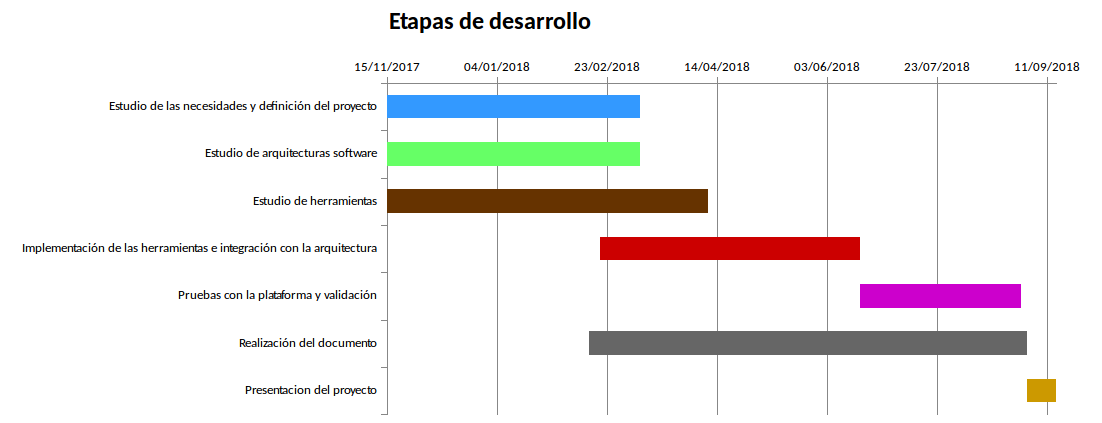
\includegraphics[scale=0.57]{Imagenes/Etapasv2.png}
\caption{Planificación del trabajo.}
\label{etapas}
\end{figure}



\section{Organización del documento\label{organizacion}}

Este trabajo se han organizado de la siguiente forma. En este primer
capítulo se ha motivado el trabajo y se han presentado los objetivos y
metodología. En el siguiente hablaremos del estado del arte, en el que
haremos un pequeño recorrido de cómo han evolucionado las plataformas
de gestión de flotas. El tercer capítulo de este trabajo se focalizará
en entender qué son y que soluciona las tecnologías que engloban el
Big Data. Tras esto, mostraremos las herramientas seleccionadas en
primera instancia y mostraremos un poco la historia de cómo surgieron.
Esto es interesante para entender por qué se han seleccionado debido
a que, evidentemente, su historia nos muestra que problemas tenían y
cómo llegaron a solucionarlo con estas herramientas. En la cuarta
parte de este trabajo, encontraremos los distintos requisitos que debe
cumplir esta prueba de concepto. Cómo grueso de este trabajo,
encontraremos el apartado de desarrollo en el cual encontraremos las
casuísticas de montar dichas herramientas sobre la arquitectura
seleccionada. En el también encontraremos el análisis de los datos que
nos ha proporcionado la empresa \mdata{} y los detalles de la
obtención de otros datos para el desarrollo de una pequeña aplicación
de monitorización del tráfico de nuestros vehículos. Para terminar con
este apartado, se explicará cómo lanzar la plataforma al detalle. Por
último, encontraremos los capítulos valoración y conclusión. En la
valoración mostraremos el grado de aceptación que ha tenido en la
empresa dicho trabajo. Por último, se presentarán las conclusiones que
hemos obtenido tras realizar dicha prueba de concepto.

%%% Local variables:
%%% TeX-master: "main.tex"
%%% coding: utf-8
%%% ispell-local-dictionary: "spanish"
%%% TeX-parse-self: t
%%% TeX-auto-save: t
%%% fill-column: 75
%%% End:
